% =============================================================================
% COPYRIGHT AND DISCLAIMER
% =============================================================================
% This file is provided as a convenience template for competition participants.
% By using it, you accept full responsibility for compliance with all applicable
% copyright, licensing, and usage rules of the Association for Computing
% Machinery (ACM) and of any LaTeX packages you load (including, without
% limitation, the "acmart" document class and related ACM materials).
%
% Consult ACM's official publication, template, and copyright policies before
% using this setup for any purpose other than this competition. Do not assume
% that this template may be reused, redistributed, or submitted elsewhere
% without independently verifying ACM's current rules.
%
% Use of the "acmart" class, the "sigconf" option, or ACM-style formatting in
% this template does NOT mean that this report, this competition, its organizers,
% or any resulting PDF is sponsored, endorsed, affiliated with, or published by
% ACM. ACM trademarks and branding remain the property of ACM.
%
% Template packages live in preamble.tex.
% Citations live in main.bib. Edit this file with your paper content.
% =============================================================================

\documentclass[sigconf]{acmart}
% =============================================================================
% Template setup — participants normally do not edit this file.
% Author content belongs in main.tex; citations belong in main.bib.
% \documentclass lives in main.tex so Overleaf does not treat this file as root.
% =============================================================================

% --- Competition / non-ACM-submission friendly rights metadata -------------
\setcopyright{none}
\settopmatter{printacmref=false}
\acmConference[Kaggle Competition]{Filament Segmentation Challenge}{2026}{\href{https://www.kaggle.com/competitions/filament-segmentation-2026}{kaggle.com/competitions/filament-segmentation-2026}}
\acmBooktitle{Competition Report}
\acmDOI{}
\acmISBN{}

% --- Author guidance text --------------------------------------------------
% \guide{...} is gray italic while \guideStyletrue; omitted from the PDF if false.
% Flip the switch in main.tex after % =============================================================================
% Template setup — participants normally do not edit this file.
% Author content belongs in main.tex; citations belong in main.bib.
% \documentclass lives in main.tex so Overleaf does not treat this file as root.
% =============================================================================

% --- Competition / non-ACM-submission friendly rights metadata -------------
\setcopyright{none}
\settopmatter{printacmref=false}
\acmConference[Kaggle Competition]{Filament Segmentation Challenge}{2026}{\href{https://www.kaggle.com/competitions/filament-segmentation-2026}{kaggle.com/competitions/filament-segmentation-2026}}
\acmBooktitle{Competition Report}
\acmDOI{}
\acmISBN{}

% --- Author guidance text --------------------------------------------------
% \guide{...} is gray italic while \guideStyletrue; omitted from the PDF if false.
% Flip the switch in main.tex after % =============================================================================
% Template setup — participants normally do not edit this file.
% Author content belongs in main.tex; citations belong in main.bib.
% \documentclass lives in main.tex so Overleaf does not treat this file as root.
% =============================================================================

% --- Competition / non-ACM-submission friendly rights metadata -------------
\setcopyright{none}
\settopmatter{printacmref=false}
\acmConference[Kaggle Competition]{Filament Segmentation Challenge}{2026}{\href{https://www.kaggle.com/competitions/filament-segmentation-2026}{kaggle.com/competitions/filament-segmentation-2026}}
\acmBooktitle{Competition Report}
\acmDOI{}
\acmISBN{}

% --- Author guidance text --------------------------------------------------
% \guide{...} is gray italic while \guideStyletrue; omitted from the PDF if false.
% Flip the switch in main.tex after \input{preamble}.
%
% Do not use \guide{...} for \email{...}.
\usepackage{xcolor}
\newif\ifguideStyle
\guideStyletrue
\newcommand{\guide}[1]{%
  \ifguideStyle
    {\color{gray!65}\itshape #1}%
  \fi
}

% --- Math ------------------------------------------------------------------
% Do NOT load amssymb (or amsfonts): acmart already loads newtxmath, which
% defines the same symbols (e.g. \Bbbk) and causes a conflict on Overleaf.
% amsmath is already provided by acmart; mathtools extends it.
\usepackage{mathtools}

% --- Figures ---------------------------------------------------------------
% graphicx is already loaded by acmart
\usepackage{subcaption}

% --- Tables ----------------------------------------------------------------
% booktabs is already loaded by acmart
\usepackage{tabularx}
\usepackage{multirow}

% --- Bibliography style is set in main.tex (ACM-Reference-Format) ----------
.
%
% Do not use \guide{...} for \email{...}.
\usepackage{xcolor}
\newif\ifguideStyle
\guideStyletrue
\newcommand{\guide}[1]{%
  \ifguideStyle
    {\color{gray!65}\itshape #1}%
  \fi
}

% --- Math ------------------------------------------------------------------
% Do NOT load amssymb (or amsfonts): acmart already loads newtxmath, which
% defines the same symbols (e.g. \Bbbk) and causes a conflict on Overleaf.
% amsmath is already provided by acmart; mathtools extends it.
\usepackage{mathtools}

% --- Figures ---------------------------------------------------------------
% graphicx is already loaded by acmart
\usepackage{subcaption}

% --- Tables ----------------------------------------------------------------
% booktabs is already loaded by acmart
\usepackage{tabularx}
\usepackage{multirow}

% --- Bibliography style is set in main.tex (ACM-Reference-Format) ----------
.
%
% Do not use \guide{...} for \email{...}.
\usepackage{xcolor}
\newif\ifguideStyle
\guideStyletrue
\newcommand{\guide}[1]{%
  \ifguideStyle
    {\color{gray!65}\itshape #1}%
  \fi
}

% --- Math ------------------------------------------------------------------
% Do NOT load amssymb (or amsfonts): acmart already loads newtxmath, which
% defines the same symbols (e.g. \Bbbk) and causes a conflict on Overleaf.
% amsmath is already provided by acmart; mathtools extends it.
\usepackage{mathtools}

% --- Figures ---------------------------------------------------------------
% graphicx is already loaded by acmart
\usepackage{subcaption}

% --- Tables ----------------------------------------------------------------
% booktabs is already loaded by acmart
\usepackage{tabularx}
\usepackage{multirow}

% --- Bibliography style is set in main.tex (ACM-Reference-Format) ----------


% Guide styling: \guideStyletrue = show gray italic hints; \guideStylefalse = omit them
\guideStyletrue
% \guideStylefalse

\usepackage{xurl}
\setlength{\emergencystretch}{2em}
\guideStylefalse
\begin{document}
\title{From solar images to filament masks}
\subtitle{A Solution to the Solar Filament Segmentation Challenge 2026}
\author{Shep Scientific}
\email{shepscientific@gmail.com}
\begin{abstract}
This report describes our solution to the Solar Filament Segmentation Challenge~2026, a Kaggle competition on automatic segmentation of solar filaments in GONG H-$\alpha$ observations.
Two stored segmentation models identify candidate filaments. A confidence-based procedure combines their masks and assigns shared pixels to one instance.
The final submission contains 1,317 masks from 180 images and has a displayed public Panoptic Quality score of 0.40.

The report explains each processing step and gives a worked mask example. Our notebook loads the exact stored weights and reproduces the submission.
\end{abstract}
\maketitle

\section{Introduction}
This report goes over the details of our submitted solution to the Solar Filament Segmentation Challenge~2026 \cite{filament-segmentation-2026}. The challenge, launched on July~10,~2026, is organized by the Earth-Space AI Research (ESAIR) Lab\footnote{\href{https://www.esairlab.com/home}{www.esairlab.com/}}. This challenge utilizes the MAGFiLO dataset for evaluation of the segmentation algorithms \cite{ahmadzadeh2024dataset}.

The pipeline converts each image into a set of filament masks. A mask is a set of pixels assigned to one object.
The model predicts a mask and a confidence score for each candidate. Post-processing turns those candidates into separate output instances.
The following sections explain the numerical operations, their purpose, and their implementation in our notebook.


\begin{figure*}[t]
\centering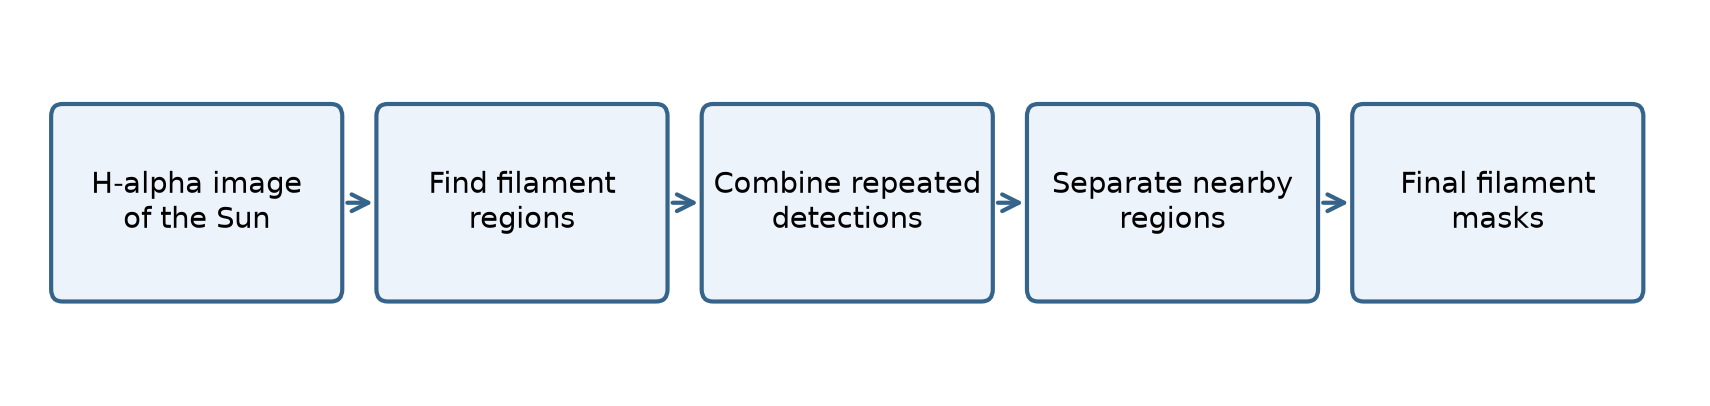
\includegraphics[width=\textwidth]{pipeline.png}
\caption{The complete inference pipeline. Each model loads our stored local weights. Mask selection and pixel assignment produce separate instances.}
\Description{One supplied image enters two models, followed by mask duplicate removal, pixel assignment, RLE encoding and validation.}
\label{fig:pipeline}
\end{figure*}

\section{Methodology}\label{sec:methodology}
\subsection{Our reproducibility package}
Our repository is \url{https://github.com/shepsci/filament-segmentation-2026-final}.
Our owned Kaggle mirror is \url{https://www.kaggle.com/datasets/shepscientific/filament-segmentation-2026-review-assets}.
The notebook uses the repository's local \path{weights/} directory. Git LFS stores the two model files.


The files are \path{yolo26x-seg-solar-filament-2048-1109.pt} and \path{yolov8x-seg-solar-filament-2048-1110.pt}.
\path{weights/manifest.json} gives their full SHA256 hashes. The loader checks each hash before model initialization.
A matching hash establishes that a reader has the same bytes used for our result.

The weights and initial inference design originate from HDJoJo~\cite{hdjojo}.
The model cards declare Apache~2.0 licensing and training on the 707 official training observations. Our contribution packages these assets and preserves valid detections from either model.
The original training cards and recovered settings are recorded in \path{provenance.json}.\footnote{The exact released files and stored settings were checked. The complete earlier initialization and training split were not independently reconstructed.}


\subsection{Prepare the image}
Each supplied JPEG has 2048 by 2048 pixels. OpenCV reads its grayscale intensity into three identical channels, as expected by the stored networks.
The predictor converts integer values in 0--255 to floating point values in 0--1 by dividing by 255.
For example, an intensity of 128 becomes approximately 0.502.


The target image dimension is 2048. The pinned Ultralytics letterbox transform keeps the aspect ratio when preparing an input.
These square images already have the target dimensions, so their geometry stays unchanged.
The predictor processes one image at a time. Its file name becomes the observation identifier in the output.


\begin{figure*}[t]
\centering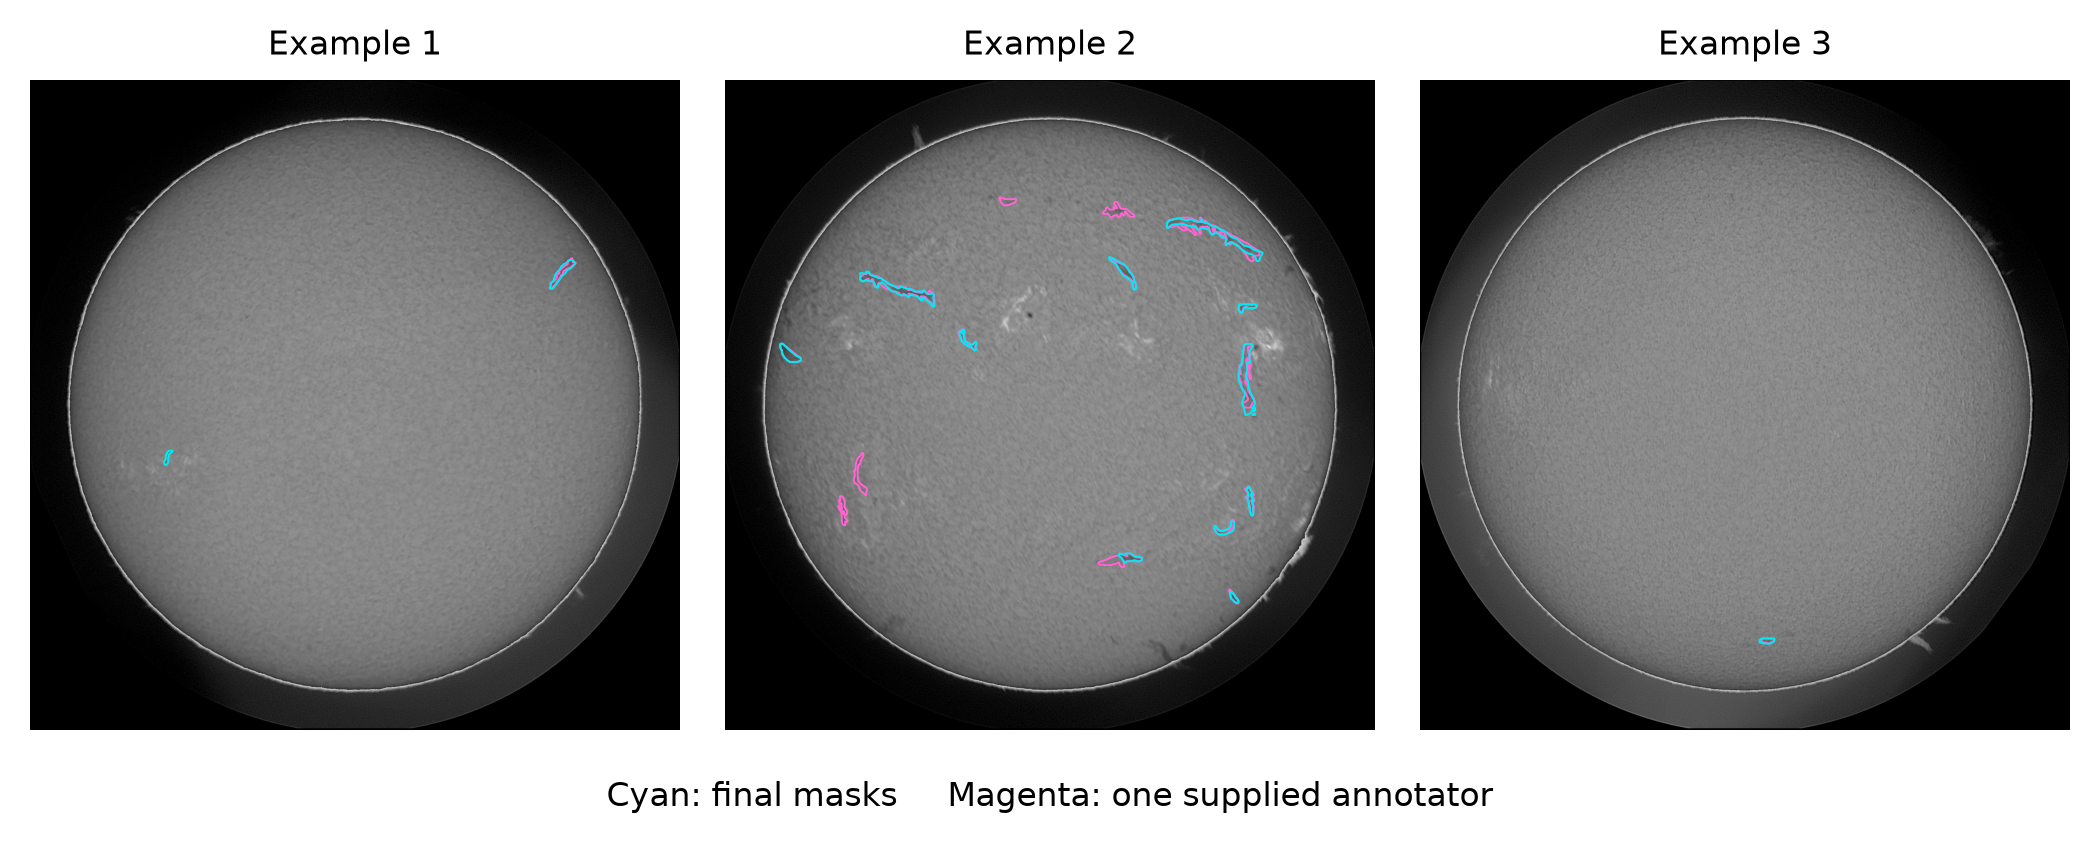
\includegraphics[width=\textwidth]{examples.png}
\caption{Final segmentations on the first three fixed diagnostic observations. Cyan shows predictions. Magenta shows one supplied annotator's masks.}
\Description{Three grayscale solar images show predicted and annotated contours, including matching regions, missed regions, and boundary differences.}
\label{fig:examples}
\end{figure*}

\subsection{Predict candidate masks}
The method uses YOLO26x-seg and YOLOv8x-seg from Ultralytics~\cite{ultralytics}.
Both are convolutional instance segmentation networks. Their first layers extract image features such as local intensity changes and edges.
Later layers combine features across spatial scales, which helps the networks represent objects with different dimensions.


The model heads use feature strides of 8, 16, and 32 pixels. A stride is the distance between adjacent feature positions in input-image coordinates.
Each segmentation head combines 32 shared mask patterns, called prototypes, with coefficients predicted for each detection.
This operation produces an instance mask together with an object location and confidence score.


YOLO26x uses C3k2 blocks and a Segment26 head. YOLOv8x uses C2f blocks and a Segment head.
Their loaded parameter counts are 70,480,895 and 71,751,811. \path{architecture.json} records the exact layer definitions and counts.
Model weights are the numerical values learned during training. The notebook loads them before prediction.


Both predictors use an image dimension of 2048, confidence threshold 0.5, and at most 100 detections.
The box-suppression IoU argument is 0.0; the end-to-end YOLO26 head retains its pinned library behavior.
Confidence places detections in a priority sequence. It should be interpreted as a ranking score rather than a guaranteed probability.


The software keeps the candidates returned by each model. This allows a filament found by one model to enter the combined result.
Each returned binary mask is resized to the input dimensions with nearest-neighbor interpolation.
Nearest-neighbor interpolation copies a nearby mask value and keeps the binary mask representation.




\subsection{Combine masks and assign pixels}
The software puts candidates in a sequence from highest to lowest confidence.
It compares each new mask with the masks already kept. Their intersection over union, or IoU, measures how much their pixel sets overlap:
\begin{equation}
\mathrm{IoU}(A,B)=\frac{|A\cap B|}{|A\cup B|}.
\end{equation}
The numerator counts shared pixels. The denominator counts pixels belonging to either mask, with shared pixels counted once.

A candidate is discarded when its IoU with any kept mask exceeds 0.5. This mask-level suppression removes strongly overlapping duplicates.
Candidates with smaller IoU can represent nearby filaments, so the software keeps them for pixel assignment.
The threshold stays fixed at 0.5 for both model sources.


Kept masks claim pixels in the same confidence sequence. A lower-confidence mask receives only pixels that a higher-confidence mask has not claimed.
This procedure gives each output pixel to at most one filament.
The software then keeps each remaining region with at least five pixels. This area check removes very small remnants after subtraction.


\paragraph{Worked example.}
Mask A contains 40 pixels and has confidence 0.90. Mask B contains 30 pixels and has confidence 0.80.
They share 10 pixels, so their IoU is $10/(40+30-10)=1/6$. Both pass mask selection.

A claims its 40 pixels first. B then keeps its 20 unclaimed pixels. The final two masks contain 60 distinct pixels.
A third candidate D has 40 pixels and shares 35 with A. Its IoU with A is $35/45$, approximately 0.778.
At confidence 0.70, D is removed as a duplicate before pixel assignment. Figure~\ref{fig:worked} shows these operations on a small grid.


\begin{figure}[t]
\centering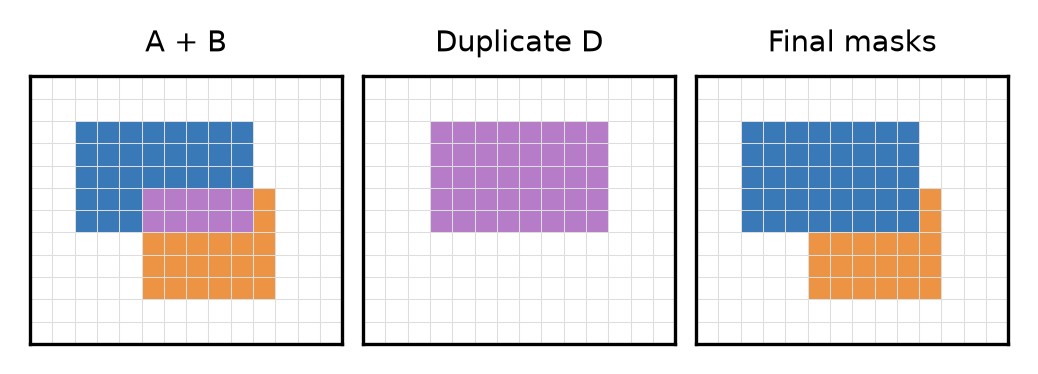
\includegraphics[width=\linewidth]{mask-worked.png}
\caption{A small mask example. A and B describe nearby regions. D duplicates A. The final grid gives shared pixels to A.}
\Description{Three colored pixel-grid panels show candidate masks A and B, duplicate D, and the separate final pixel assignments.}
\label{fig:worked}
\end{figure}

\subsection{Encode and check the output}
Pycocotools converts each final mask to compressed COCO run-length encoding, or RLE.
RLE stores runs of pixels rather than listing all pixel values.
The CSV has two fields: \path{filament_id} and \path{segmentation_rle}. Each predicted filament receives one row and a unique identifier.


Output checks decode the masks and confirm their 2048 by 2048 dimensions, nonempty regions, identifiers, and pixel separation.
An image with no predicted filament produces no rows. The pipeline still records that the image was processed.
These checks make the encoded output suitable for the competition's instance evaluation.


\subsection{Training record and optional learning path}
The submitted networks use the released weights. Their declared training source contains 707 observations, 1,154 annotator records, and 8,199 masks.
Recorded training settings include image dimension 2048, batch size 8, MuSGD, initial learning rate 0.001, and weight decay 0.0001.
The maximum epochs are 500 and 300, with early stopping patience of 25 and 30 for YOLO26x and YOLOv8x.


The stored arguments also describe rotation, translation, scaling, shear, and horizontal and vertical flips.
\path{provenance.json} records the complete recovered argument lists.
This distinguishes the training configuration from the fixed prediction settings explained above.

For readers who want to train a new model, the notebook includes an optional procedure in \path{train.py}.
It exports the supplied instance polygons into one filament class and starts from the recorded architecture.
It groups every annotator record of an observation into the same data split.


A fixed SHA256 ordering assigns 566 observations to training and 141 to validation. Grouping prevents copies of one observation from entering both sets.
The optional procedure records its seed, optimizer, augmentation settings, and split manifest. It is a new training recipe, distinct from the released weights' history.
The default notebook path loads the stored final weights and runs inference.


\section{Evaluation}\label{sec:evaluation}
\subsection{Final competition result}
The selected submission, 58351849, has a displayed public Panoptic Quality score of 0.40.
The pipeline processed all 180 supplied test images. It produced 1,317 masks in 178 images, with two images having no masks.
Every output pixel belongs to at most one predicted instance.


A second complete notebook execution reproduced the submitted CSV byte for byte on Apple MPS.
The file hash and validation receipt are included in our package. The displayed public score describes the public leaderboard portion of the test set.
The private score remains unavailable.


\subsection{Read the diagnostic measures}
Panoptic Quality, or PQ, combines finding the correct instances with matching their shapes.
A matched pair has IoU above 0.5. An extra prediction is a false positive; a missed reference instance is a false negative.
The score divides the sum of matched IoUs by $TP+0.5FP+0.5FN$.


Dice and IoU also describe overlap between the union of predicted pixels and an annotator's union mask.
We report their means and per-record distributions in the evaluation output.
One-to-many counts describe a reference instance split across several predictions. Many-to-one counts describe predictions that merge reference instances.


\subsection{Final method and component baselines}
We compare the final configuration with each individual model on a fixed diagnostic set.
It contains 12 official training observations and their 17 annotator records. The selection rule sorts observation names by \texttt{SHA256(final-method-diagnostics-v1:name)}.
This rule selects the examples before inference scores are available.


These are training-set diagnostics because the released weights have seen the training observations. They illustrate behavior and do not estimate held-out performance.
The evaluator scores each annotator record with the observation's predictions, following the host self-evaluation notebook~\cite{hosteval}.
PQ counts are pooled across those records.


\begin{table}[t]
\caption{Fixed training-set diagnostics. Dice and IoU are mean binary-mask scores. PQ intervals show observation sampling uncertainty.}
\label{tab:diagnostics}
\centering\small
\begin{tabular}{lccc}\toprule
Method & PQ [95\% interval] & Dice & IoU\\\midrule
YOLO26x & 0.488 [0.396, 0.565] & .565 & .432\\
YOLOv8x & 0.517 [0.418, 0.626] & .615 & .474\\
Final ensemble & 0.531 [0.448, 0.619] & .687 & .538\\\bottomrule
\end{tabular}
\end{table}

The final method matches 98 reference pairs, compared with 77 and 90 for the individual models.
It has 30 extra predictions and 34 missed instances. The individual models have 10/55 and 26/42 extra/missed instances.
These counts show the coverage tradeoff when combining detections.


The final matched-instance IoU has mean 0.704 and median 0.721. Its 10th and 90th percentiles are 0.585 and 0.804.
At a diagnostic overlap threshold of 0.1, the result has zero one-to-many cases and three many-to-one cases.
This lower threshold describes partial overlaps that can reveal splitting and merging.


Confidence intervals use 2,000 bootstrap samples with seed 3407. Each sample resamples whole observations and keeps their annotator records together.
This respects the shared image behind multiple annotation records. The interval describes sample variability; training reuse still limits generalization claims.
The evaluation module and recorded metrics reproduce these calculations.




\subsection{Strengths, limits, and reuse}
Combining two models can recover candidates found by either network. Mask suppression reduces duplicates, while pixel assignment preserves separate output instances.
Figure~\ref{fig:examples} shows how predicted boundaries compare with supplied annotations.
The examples include both agreements and differences.


Small or faint filaments can be missed. Nearby instances can merge, and extra candidates can increase the false-positive count.
The fixed diagnostic set is small, so its results should be read with the uncertainty intervals.
A useful next step is observation-grouped validation of a newly trained model, with explicit attention to boundaries and merged instances.


The recorded environment uses Python 3.12.12, Ultralytics 8.4.212, PyTorch 2.13.0, torchvision 0.28.0, and NumPy 2.5.2.
It uses OpenCV 5.0.0.93 and pycocotools 2.0.11. \path{requirements.txt} lists all package versions.
Exact replay was verified on Apple MPS. Numerical differences near thresholds can change results on other hardware.


Readers can use the notebook in three ways: reproduce the final predictions, inspect diagnostic measures, or learn the optional new training workflow.
Reusable modules implement inference, evaluation, and training. The notebook explains their inputs, numerical decisions, and outputs.
All prediction dependencies are stored in our repository. The official competition distribution supplies the image inputs.


\section{Acknowledgment}\label{sec:acknowledgment}

    % Do not change
    The organization of the Filament Segmentation Challenge 2026 is partially supported by the U.S. National Science Foundation (NSF) under Grant No. 2209912 and 2433781, directorate for Computer and Information Science and Engineering (CSE), and Office of Advanced Cyberinfrastructure (OAC), and Grant No. 2511630, AST Division Of Astronomical Sciences and MPS Directorate for Mathematical and Physical Sciences.

    The Filament Segmentation Challenge 2026 is sponsored by the U.S. National Science Foundation (NSF) National Solar Observatory (NSO). 

    This work utilizes GONG data obtained by the NSO Integrated Synoptic Program, managed by the National Solar Observatory, which is operated by the Association of Universities for Research in Astronomy (AURA), Inc. under a cooperative agreement with the National Science Foundation and with contribution from the National Oceanic and Atmospheric Administration. The GONG network of instruments is hosted by the Big Bear Solar Observatory, High Altitude Observatory, Learmonth Solar Observatory, Udaipur Solar Observatory, Instituto de Astrofísica de Canarias, and Cerro Tololo Interamerican Observatory.


\bibliographystyle{ACM-Reference-Format}
\bibliography{main}
\end{document}
